
\documentclass[12pt]{article}
%	options include 12pt or 11pt or 10pt
%	classes include article, report, book, letter, thesis

\usepackage[margin=0.5in]{geometry}

\setlength{\parindent}{0pt}

\usepackage{hyperref}
\usepackage{graphicx}

%for writing of code in blocks like
%\begin{lstlisting}
%   .......
%\end{lstlisting}
\usepackage{listings}
\usepackage{color}
\usepackage{enumitem}

\definecolor{dkgreen}{rgb}{0,0.6,0}
\definecolor{gray}{rgb}{0.5,0.5,0.5}
\definecolor{mauve}{rgb}{0.58,0,0.82}

\lstset{frame=tb,
  language=C++,
  aboveskip=3mm,
  belowskip=3mm,
  showstringspaces=false,
  columns=flexible,
  basicstyle={\small\ttfamily},
  numbers=none,
  numberstyle=\tiny\color{gray},
  keywordstyle=\color{blue},
  commentstyle=\color{dkgreen},
  stringstyle=\color{mauve},
  breaklines=true,
  breakatwhitespace=true,
  tabsize=3
}
%%%%%%%%%%%%%%%%%%%%%%

\title{Life of a Particle : Assignment 3}
\author{Sam Meehan}
\date{Due Date : 20 January 2017}

\begin{document}
\maketitle

\textbf{How to Submit}
\newline
This assignment should be submitted by replying to the email sent out by the tutors - \textbf{Use the online form!} - with the link to your GitHub repository.  Contained within this repository should be a \href{https://github.com/adam-p/markdown-here/wiki/Markdown-Cheatsheet}{markdown README.md} file which provides a guide to the contents of the repository, along with instructions of how to run the code, where necessary.  For the full assignment, also include a well-written summary in the form of a latex document with one section per question.
\newline
\newline
\textbf{You are to work with the group assigned to you by the tutors.}
\newline
\newline
\textbf{Calculating $\pi$} 
\newline
\newline
This question was started in class.  The aim is to calculate the value of $\pi$ using Monte Carlo integration.  Here is a brief review of the algorithm (which can be found on the internet in many places) :
\begin{itemize}[noitemsep]
\item Generate a large number $N$ of $(x,y)$ pairs that bound a quarter circle of radius $R$ in quadrant 1.
\item Determine the fraction of these pairs that fall within the circle : $f_{in}=N_{in}/N$.
\item Relate this fraction to the area of the circle ($A_{circle}=\frac{1}{4}\pi R^2$) compared to the area of the bounding box ($A_{box}=R^2$) as $f_{in}=A_{circle}/A_{box}=\frac{1}{4}\pi$
\item Relate the value of $\pi$ directly to the fraction of points within the circle : $\pi=4f_{in}$
\end{itemize}
Now, the possible values of $f_{in}$ will depend on the initial number of points that were generated ($N$) and what we are interested in is knowing both how to calculated value of $\pi$, and the related statistical uncertainty, vary as $N$ is increased.
\newline
\newline
To get a handle on this, calculate the value of $\pi$ some large number of times $M$ for a fixed value of $N$.  For each one of these $M$ calculations, store the value of $\pi$ that you determine.  After all $M$ calculations, determine the mean and standard deviation of this set of numbers (which can be visualized as a histogram).  You now have $\pi(N)$ and $\sigma_{\pi}(N)$.  Perform this procedure for increasing values of $N$.  How do these two values ($\pi(N)$ and $\sigma_{\pi}(N)$) evolve as $N$ increases.
\newline
\newline
\textbf{The Classical Particle In a Box} 
\newline
\newline
Before writing a simulation to describe the quantum particle in a box, it is important to be able to accurately describe the \textit{classical} particle in a box.  To do this, imagine the following experimental setup.  You place a particle in a box of width $a$ on the left side (at $x=$0) with some fixed velocity $v$ that will cause it to move towards the right.  You then immediately close your eyes.  When the particle reaches the right hand side, you know that it will immediately reverse direction and travel back to the left.  This process will continue with the particle bouncing from one side to the other for a time $T$ (with $T>>a/v$) at which point you open your eyes and note the current position $x$ of the particle.  This measurement constitutes one experiment.
\begin{figure}[h!]
  \center
  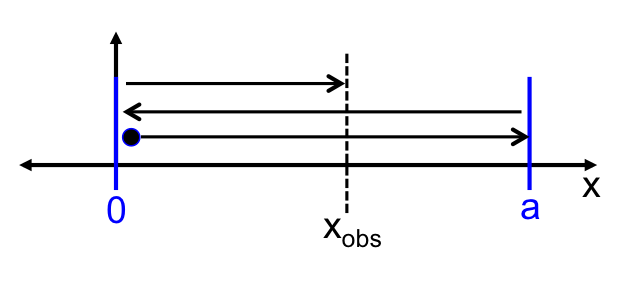
\includegraphics[width=0.5\linewidth]{classical.png}
  \caption{The experimental setup for one trial of the classical particle in a box.  The ball is released, it bounces back and forth a few times and after waiting a time $T$, you open your eyes and observe it at $x=x_{obs}$.}
  \label{fig:riemann}
\end{figure}
Imagine that you repeat this same experiment many many times. What will be the distribution of the ensemble of $x_{obs}$ values?  Your task in this question is to design a simulation that produces this distribution.
\newline
\newline


\textbf{Modelling the Particle In a Box} 
\newline
We discussed at great length the solution of the Schrodinger equation for the case of a particle in a one-dimensional box with sides at $x=$0 and $x=$a (Go review \href{http://www.fisica.net/mecanica-quantica/Griffiths\%20-\%20Introduction\%20to\%20quantum\%20mechanics.pdf}{Griffith's QM - Chapter 2.2} if you are not sure of how the calculation proceeds.).  This is the model by which we want to describe a particle, namely the answer to the question ``Where is the particle?''.  This will be done using the wave function $\Psi(x,t)$ of the particle, which itself may be complex valued as is composed as a linear superposition of the eigenfunctions 
\begin{displaymath}
 \Psi(x,t)=\displaystyle\sum_{n=0}^{\infty} c_{n}  \phi_{n}(t)  \psi_{n}(x) = \displaystyle\sum_{n=0}^{\infty} c_{n}  e^{-\frac{i}{\hbar}E_{n}t} sin(\frac{n\pi}{a}x)
\end{displaymath}
However, the probability rule, which will be a function describing the PDF $P(x)$ of the location of the particle, must be a real valued function from which a single event (a single collapse of the wave function) can be viewed as the generation of a single number from this distribution $P(x)$.  Therefore, we must translate this complex function into a real-valued function.  Two reasonable ways to do this are :
\begin{itemize}
\item Square Then Sum : Take the square modulus of each of the eigenfunctions and then add these squared terms.
   \begin{itemize}
     \item $P_{A}(x,t)=\displaystyle\sum_{n=0}^{\infty}  c_{n}  \phi_{n}(t)  \psi_{n}(x) c_{n}^{*}  \phi_{n}^{*}(t)  \psi_{n}^{*}(x) $
   \end{itemize}
\item Sum Then Square : Add the individual eigenfunctions and then take the square modulus of this sum.
   \begin{itemize}
     \item $P_{B}(x,t)=\displaystyle\sum_{n=0}^{\infty}  c_{n}  \phi_{n}(t)  \psi_{n}(x) \times \displaystyle\sum_{m=0}^{\infty}  c_{m}^{*}  \phi_{m}^{*}(t)  \psi_{m}^{*}(x)$
   \end{itemize}
\end{itemize}

If you are feeling overwhelmed looking at these equations,its alright, we are going to deal with a simplified system.  Let's imagine that we know that the particle is initially placed in the box in a state $\Psi(x,t)$ which is only composed of the $E_1$ and $E_2$ eigenstates.  So the wave function is simply 
\begin{displaymath}
\Psi(x,t)=c_{1}\phi_{1}(t)\psi_{1}(x)+c_{2}\phi_{2}(t)\psi_{2}(x)
\end{displaymath}
First, describe how these two different possibly probability rules differ (if they do) qualitatively?  Is there time dependence to one of the probability rules?  What if you set $t=$0, meaning that the observation is made immediately after you put the particle in the box?  Does the time dependence go away?
\newline
\newline
For this simplified system, you have been provided with a set of 10000 data measurements (included in the GitHub - \href{https://github.com/smeehan12/LifeOfAParticle/tree/master/Assignments/assignment3/particle_in_a_box_v0_PerfectDetector_N10000.txt}{Link to GitHub Assignment3 data file}).  If you feel that you need more data points to be able to successfully carry out the assignment, please ask.  Your goal is to determine which one of these two probabily rule transformations $P_{A}$ or $P_{B}$ is the one that really occurs in nature.  To this end, you should probably start by examining the data, either by using descriptive statistics, or maybe making a histogram.  Can you observe anything about the data just from this?  Now try to generate a predictive set of data according to the two different models that you have for the probability, assuming that the measurements being made are performed immediately at $t=$0.  
\newline
\newline
To fully describe the model, there are therefore two separate questions to answer
\begin{itemize}[noitemsep]
\item What is the probability rule that comes from nature?
\item What are the coefficients $c_1$ and $c_2$? (To make things less involved, pretend that we know that $c_1$ and $c_2$ are positive and between [$0,1$].)
\end{itemize}
To go about this, we will need a way to compare your ensemble of predictions to that of the observations.  This can be done by first casting the obervations or predictions in the form of two histograms ($p$ and $o$) and then performing a calculation of the $\chi^{2}$ of these two histograms where
\begin{displaymath}
\chi^{2}=\displaystyle\sum_{i \in bins(p,o)} \frac{(p_{i}-o_{i})^2}{\sigma_{p_{i}}^{2}+\sigma_{o_{i}}^{2}}
\end{displaymath}
and ($p_{i}$, $o_{i}$) is the bin content of $p$ and $o$ at bin $i$ and ($\sigma_{p_{i}}$, $\sigma_{o_{i}}$) are the corresponding errors on these bins.  When creating a histogram of the number of events in a bin ($N_{i}$), the ROOT package will automatically set the error on the bin to be the square root of this value ($\sqrt{N_{i}}$).  This is on account of the fact that the number of events in a bin is viewed as a poisson observable.  That is, if you were to run the simulation again and again, each time obtain another count of events in bin $i$, and you were to make a histogram of these values, then it would follow a poisson distribution of mean $N$ and standard deviation $\sqrt{N}$ (\textit{BONUS} points if you do this and justify the error being $\sqrt{N}$. 
\newline
\newline
\textbf{Modelling a \textbf{Real Life} Particle In a Box - \textit{Bonus/Optional}} 
\newline
This problem builds upon the previous problem to incorporate effects of a real particle detector.  You will again be given a set of data, with the goal to measure the $c_1$ and $c_2$ coefficients.  Hopefully you have discovered the probability rule from the previous question so that will not be necessary again.  The challenge this time will be to properly take into account detector effects.
\newline
\newline
In the previous problem, when the wave function collapsed and produced an $x$ position, we assumed that the measured position of this particle corresponded exactly to its \textit{actual} position.  However, in a real experiment, the manner in which the measurement of a position (or really any attribute of a particle) is imperfect.  These imperfections are often caused by experimental noise within the detector that can cause the observed position to deviate slightly from the position where the particle ``really'' was.  These imperfections are completely analagous to the imperfections which exist within the eyes of people who must wear glasses.  Typically, light entering a normal eye would indicate where the object from which that light comes is located.  However, if your eyesight is not 20:20, then when the light enters the eye, it becomes smeared out by these abberations and the resulting image in the eye becomes blurry.  The same occurs in imperfect (read: real) particle detectors.  Because of noise, when a particle enters the detector it can get shifted.  If we take an ensemble of such particles all entering the same location, then they will become smeared out in a random fashion.  By this, we mean that on a particle-by-particle basis, the shift which occurs is random and distributed according to what is called the ``point spread function'' of the detector.    The point spread function can be interpreted as a PDF of the shift in the position of the measurement with respect to the actual position of the particle upon measurement.  Therefore, if the true position before measurement is $x_{true}$ then the measured position will be $x_{meas}$=$x_{true}+x_{shift}$ where $x_{shift}$ is a random number drawn from the point spread function.
\begin{figure}[h!]
  \center
  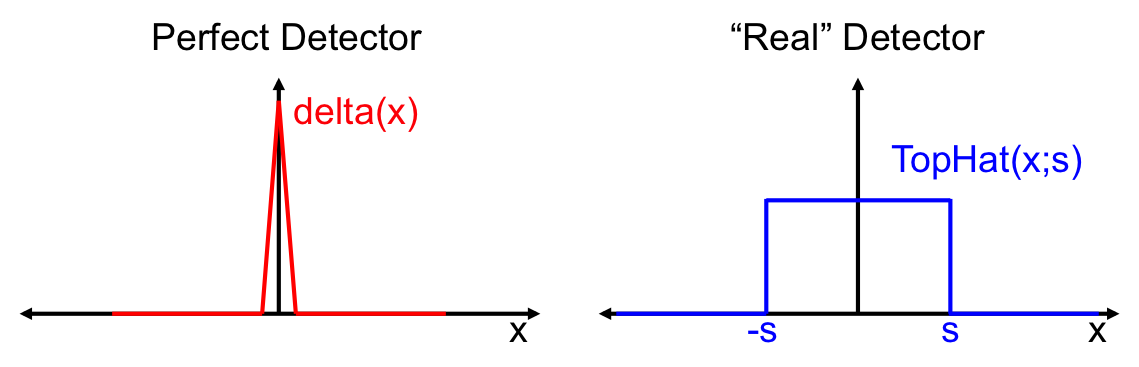
\includegraphics[width=0.8\linewidth]{detector.png}
  \caption{The point spread function for a perfect detector (left) and a real detector (right).  The point spread function for the position measurement represents the PDF of the shift in the position of the measurement with respect to the actual position of the particle upon measurement.}
  \label{fig:riemann}
\end{figure}
\newline
\newline
In addition to the measurement being obscured by the smearing of the true position to the final measured position, another common effect is detector \textit{inefficiency}.  This comes about again by imperfections in the detector and also ``thresholds'' that must be set by the experimentalist to suppress noise.  However, what these contribute to is a non-unity probability to observe a particle that enters the detector.  In other words, when the wave function collapses and a particle is to be observed at some position in the detector, then there is a finite probability $\epsilon\leq 1$ that the particle is actually observed.  This means that if you were to ``shoot'' 100 particles into the detector and $\epsilon=0.73$ then you would only observe 73 of them.  
\newline
\newline
For this question, we want to take into consideration these two effects to model the set of data coming from the real detector.  
\begin{itemize}[noitemsep]
\item Smearing : $x_{meas}$=$x_{true}+x_{shift}$ where $x_{shift}$ is distributed according to the point spread function
\item Inefficiency : There is an efficiency $\epsilon\leq 1$ for observing the particle if it enters the detector.  
\end{itemize}
The detector system that we have constructed to observe our particle in the box consists of two detectors as indicated.  The first detector covers the first half of the box [0,$a/2$) and the second detector covers the second half [$a/2$,$a$].  Each detector has its on imperfections and may have different smearing or inefficiencies, both of which may need to be taken into account for both detectors.
\begin{figure}[h!]
  \center
  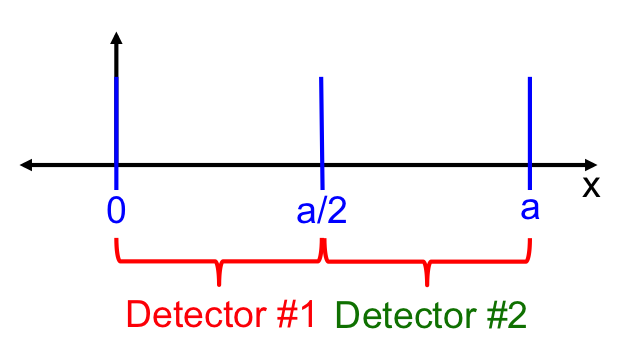
\includegraphics[width=0.4\linewidth]{setup.png}
  \caption{The setup of our particle in the box experiment.}
  \label{fig:riemann}
\end{figure}
\newline
\newline
Your challenge is to build a model which accurately describes the observed ensemble of data and measure the $c_1$ and $c_2$ coefficients using a similar technique as before ($\chi^2$ minimization).  However, in this case there are four additional free parameters
\begin{itemize}[noitemsep]
\item $s_{1}$ : The magnitude of the smearing in Detector \#1
\item $\epsilon_1$ : The efficiency of Detector \#1
\item $s_{2}$ : The magnitude of the smearing in Detector \#2
\item $\epsilon_2$ : The efficiency of Detector \#2
\end{itemize}
You can go about this in any way you want, by either performing a $\chi^2$ minimization over all the parameters (might be slow), or by examining the data and trying to find an alternative way to estimate the $s_i$ and $\epsilon_i$ parameters using a combination of qualitative and analytical arguments.  There is no single approach that works better than any other, but you can be assured that the $c_1$ and $c_2$ coefficients are not the same as before.
\end{document}




